\section{Problem 4-3 Network Measures of Real Graphs}

See \textit{problem\_3.ipynb}.

\begin{enumerate}
	\item The diameter of the largest connected component is 15.
	\item The node with the highest degree hast the ID 2332 and a degree of 1098.
	\item The number of triangles in the network is 3501542.
	\item The global clustering coefficient of the network is 0.22099367691190397.
	\item The power-law exponent of the degree distribution is 0.79...  which is wrong.  It should be arround 1.43
	\item See the following figure:
	
	\begin{figure}[h]
		\centering
		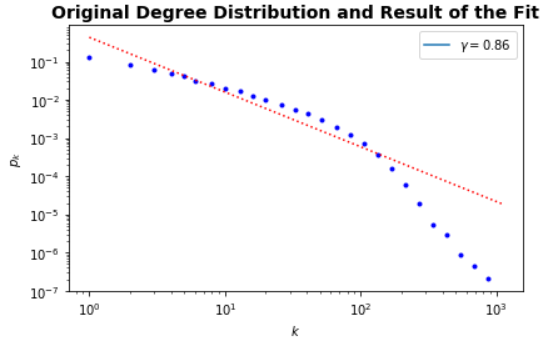
\includegraphics[width=0.9\linewidth]{images/problem43_degree_distribution.png}
		\caption{Real and fitted degree distribution of facebook links.}
		\label{distribution}
	\end{figure}
\end{enumerate}

